\newcommand{\outlierFig}{
  \begin{figure}
  \centering
  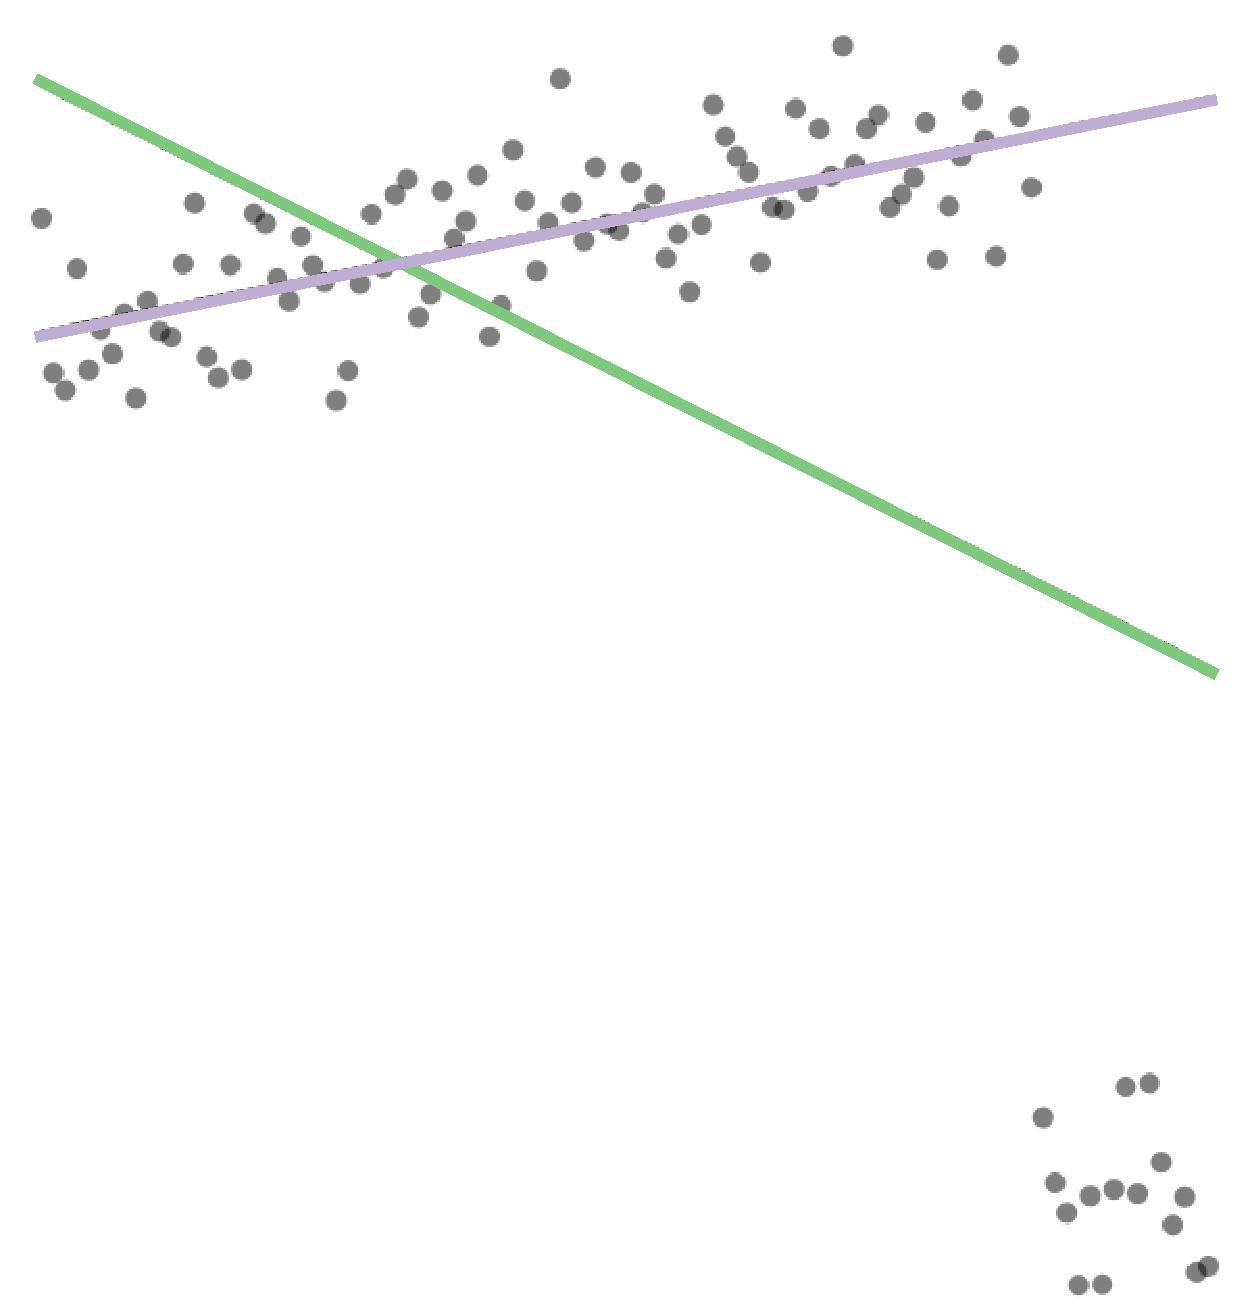
\includegraphics[width=.55\columnwidth]{figures/exp4}
  \caption{An example stimulus from experiment 3. We replaced the final 10 points of this dataset with extreme values. The overlaid green trend line represents a robust fit (ignoring the outlier values), while the overlaid orange line represents the standard OLS fit with all points included. The purple line represents the average participant response on this stimulus. In general, participants' estimates of trend lines were closer to the robust than the non-robust trend; regression by eye tends to underweight outliers compared to OLS.}
  \label{fig:outlier}
  \end{figure}
}

\newcommand{\expFig}{
  \begin{figure}
  \centering
  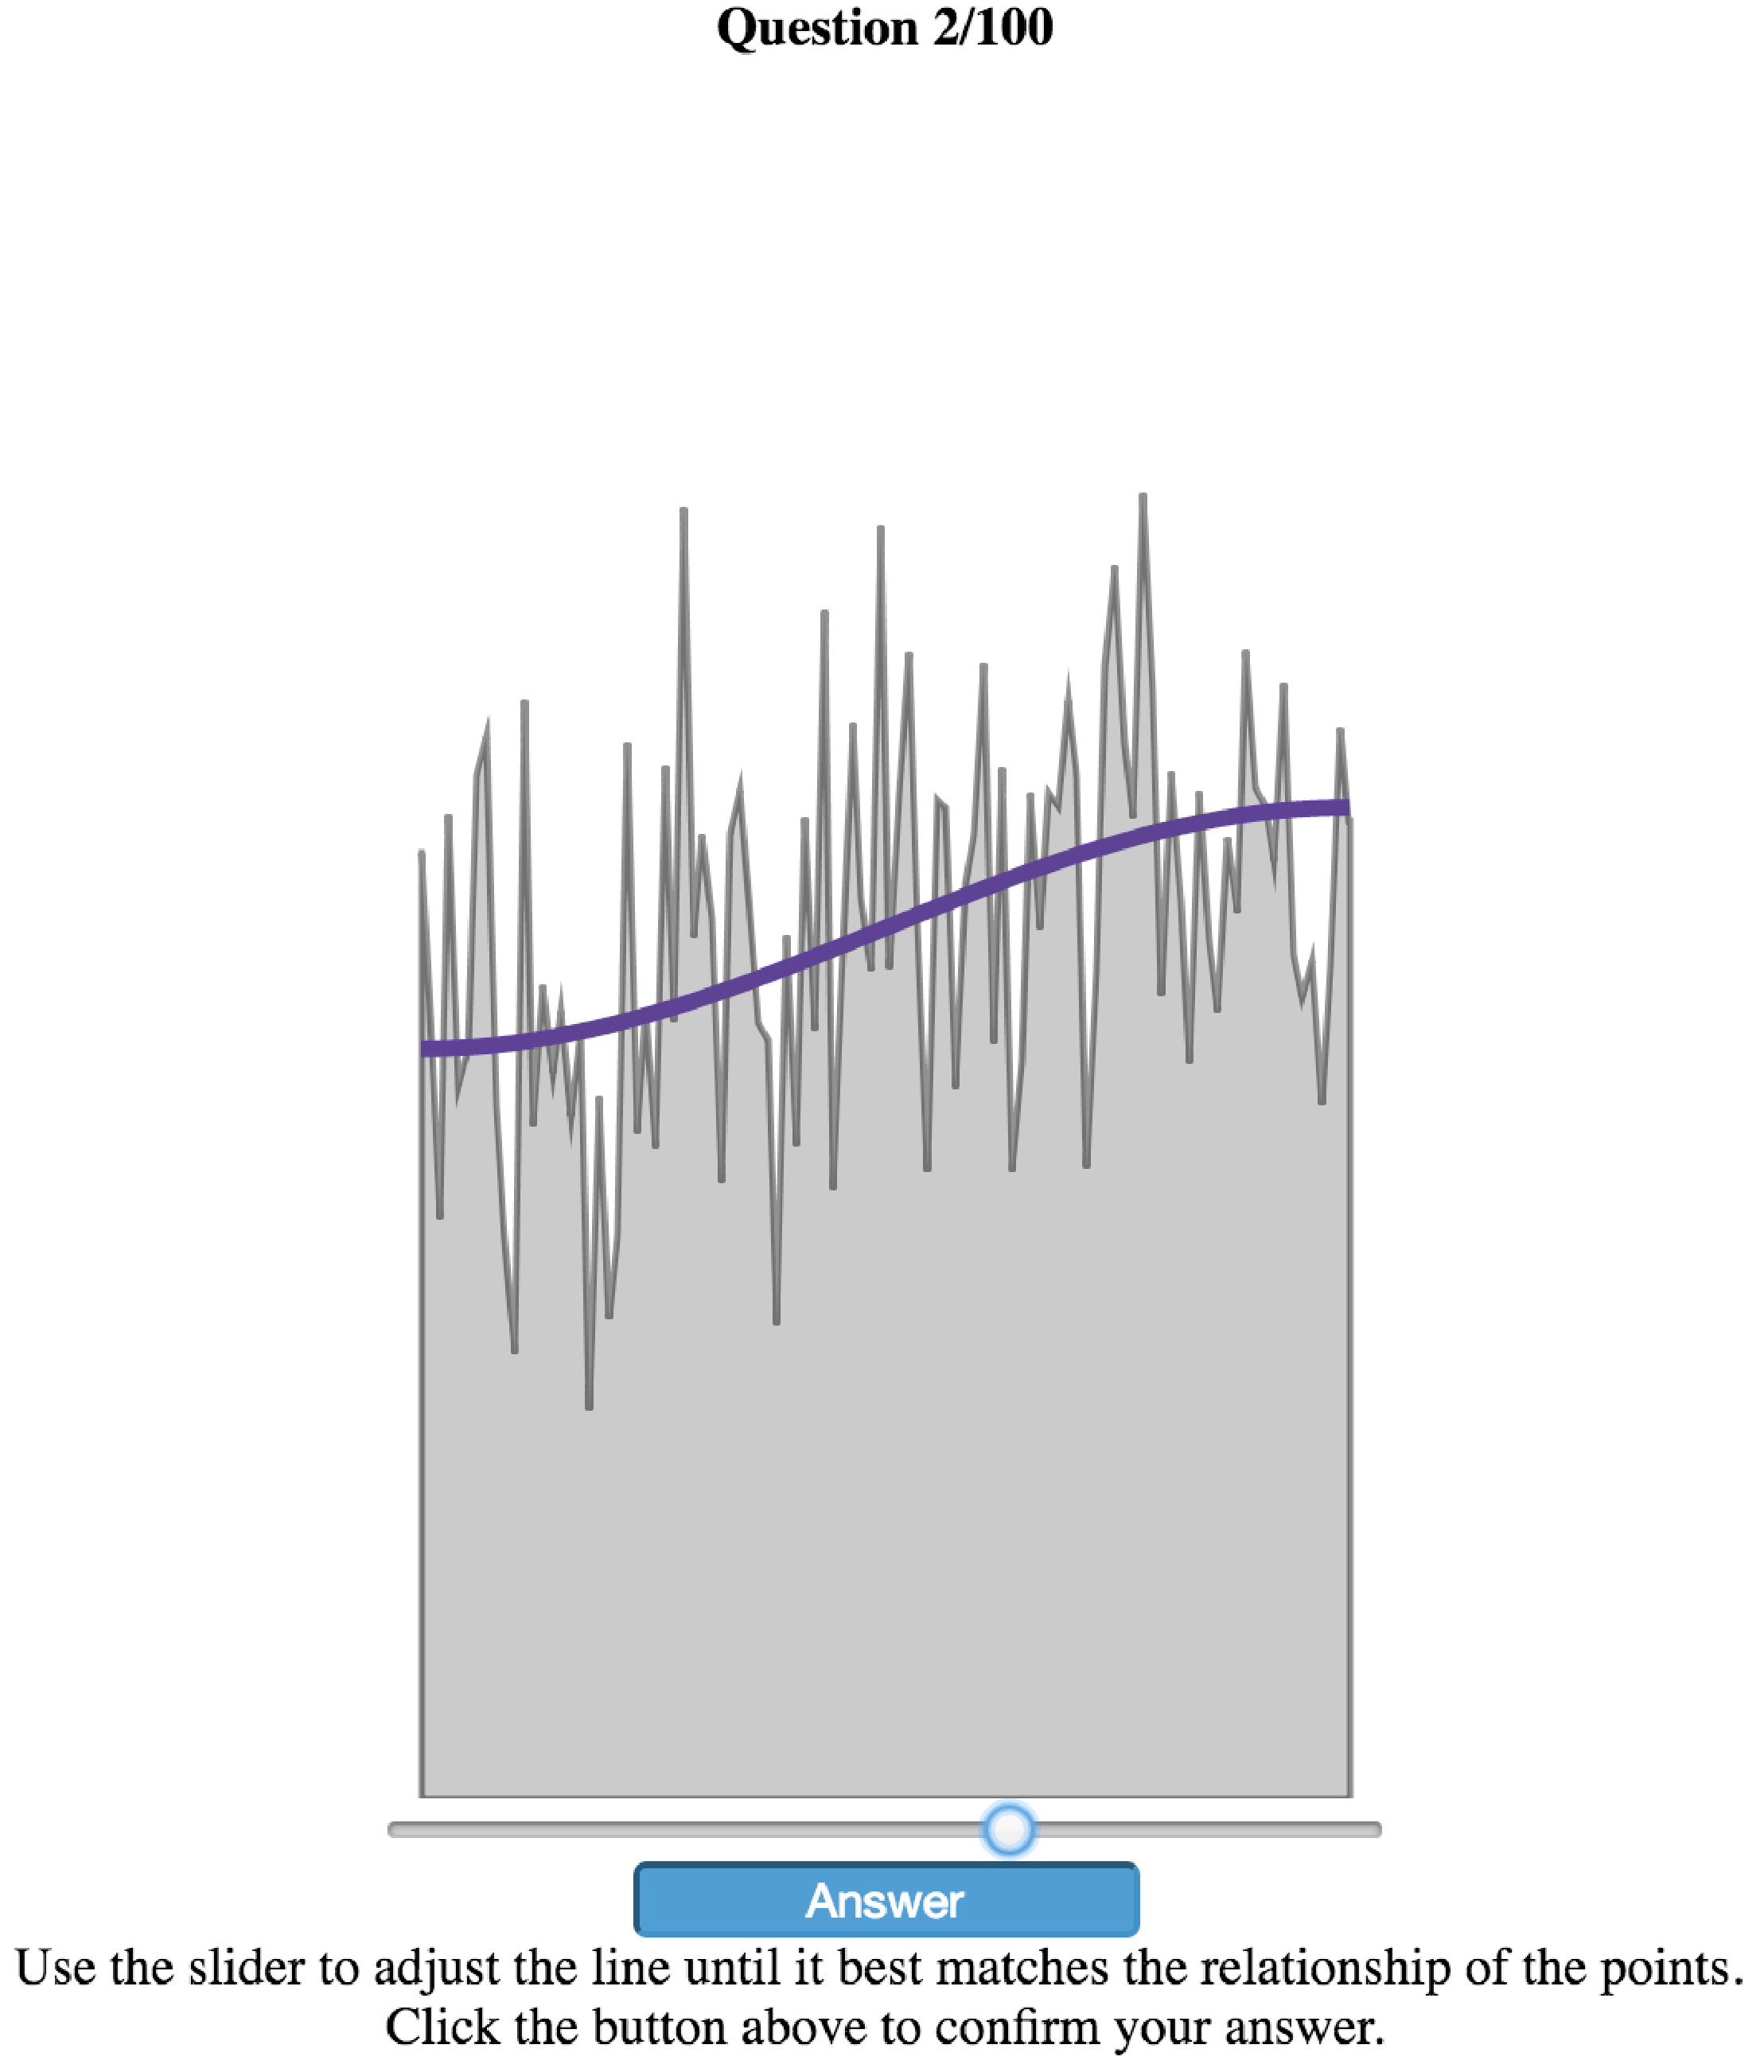
\includegraphics[width=.65\columnwidth]{figures/exp}
  \caption{An example estimation task from our experiments. Here, the participant must adjust the amplitude of the purple trigonometric function until it best matches a particular set of bivariate data.}
  \label{fig:experiment}
  \end{figure}
}

\newcommand{\anscombeFig}{
	\begin{figure*}
		\centering
		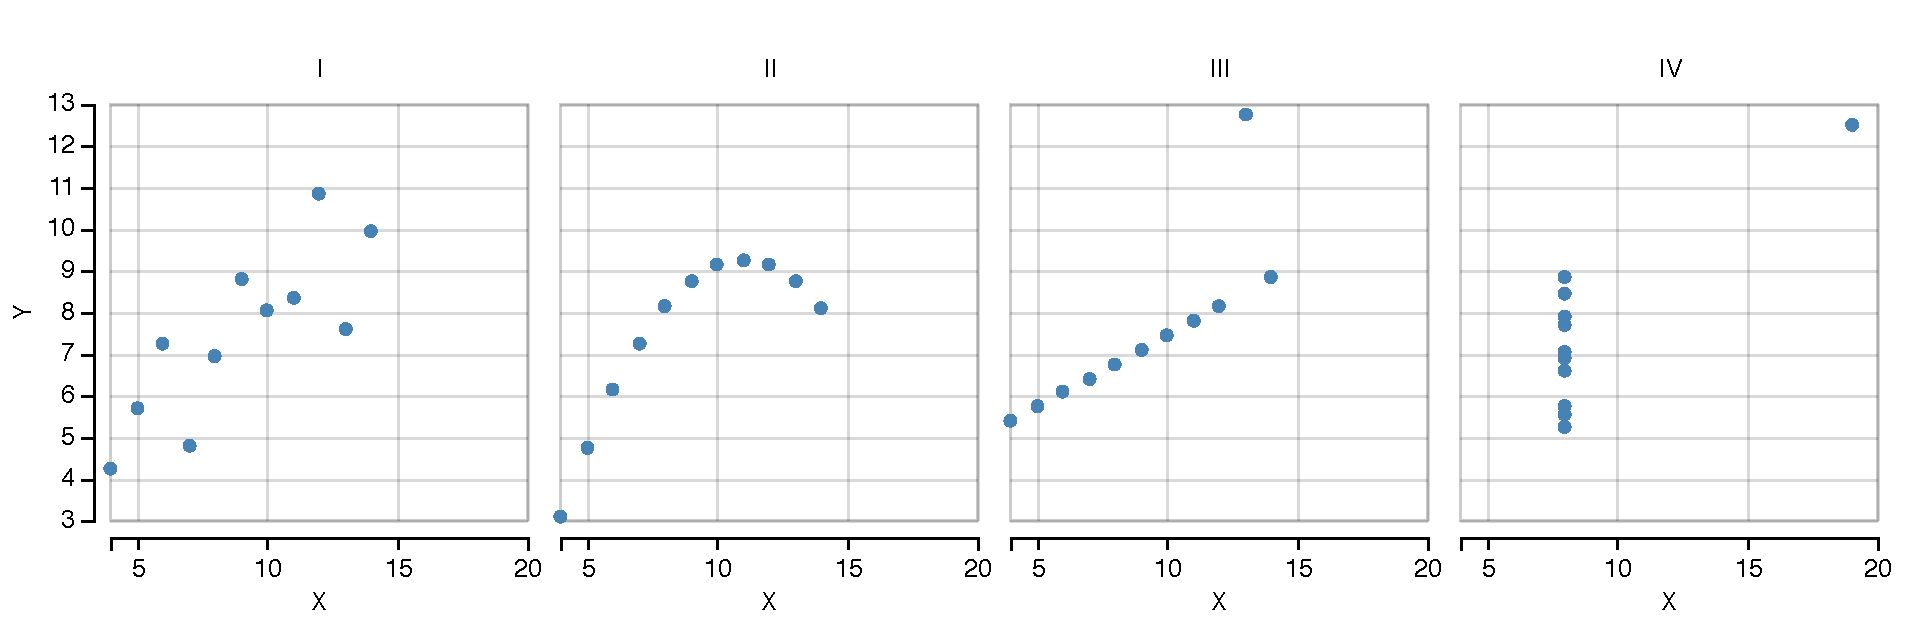
\includegraphics[width=.75\textwidth]{figures/anscombe}
		\caption{Anscombe's quartet. Each series has nearly identical summary statistics include mean, standard deviation, and linear fit. Yet, viewers can disambiguate, through visual inspection, differing patterns and trends. We refer to this visual estimation of trend as ``regression by eye.''}
		\label{fig:anscombe}
	\end{figure*}
}

\newcommand{\sigmasFig}{
	\begin{figure}
		\centering
		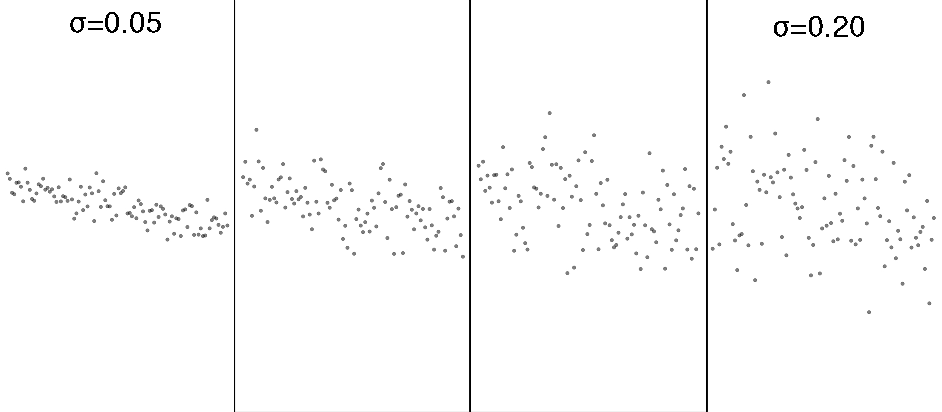
\includegraphics[width=.95\columnwidth]{figures/sigmas}
		\caption{The effect of increasing residual bandwidth on stimuli. We produced stimuli by creating points on a target trend line (in this case, $f(x) = -0.2x + 0.6$), and then adding residuals drawn evenly from a gaussian with a given bandwidth $\sigma$. Larger bandwidths mean more dispersion and so weaker fits.}
		\label{fig:sigmas}
	\end{figure}
}

\newcommand{\expOnesigmasFig}{
	\begin{figure}
		\centering
		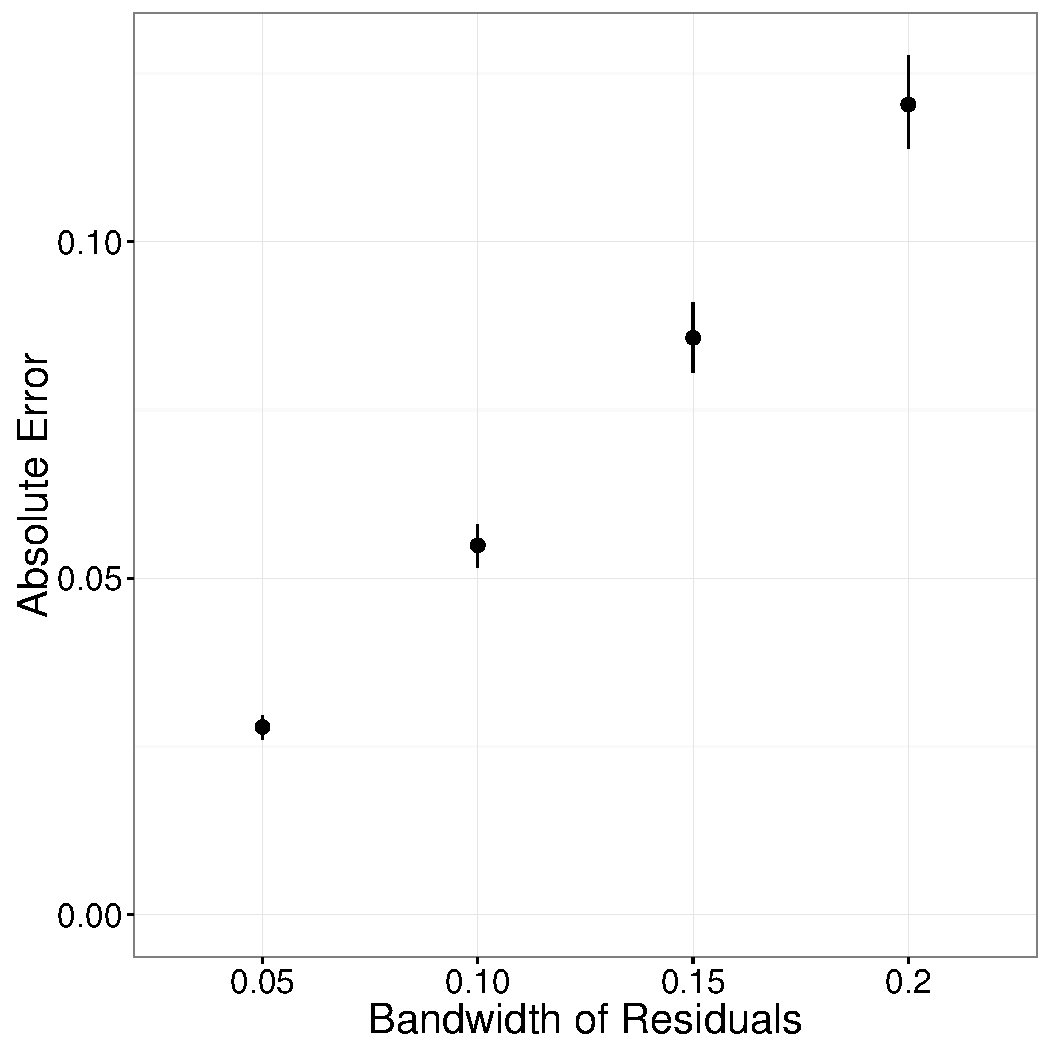
\includegraphics[width=.85\columnwidth]{figures/exp1sigmas}
		\caption{From experiment 1, the effect of increased residual bandwidth on error. See Fig. \protect\ref{fig:sigmas} for example stimuli at each factor level. Absolute error at estimating trend monotonically increases as the goodness of fit decreases. Confidence intervals represent bootstrapped 95\% c.i.s of interquartile mean. }
		\label{fig:exp1sigmas}
	\end{figure}
}

\newcommand{\typesFig}{
	\begin{figure}
		\centering
		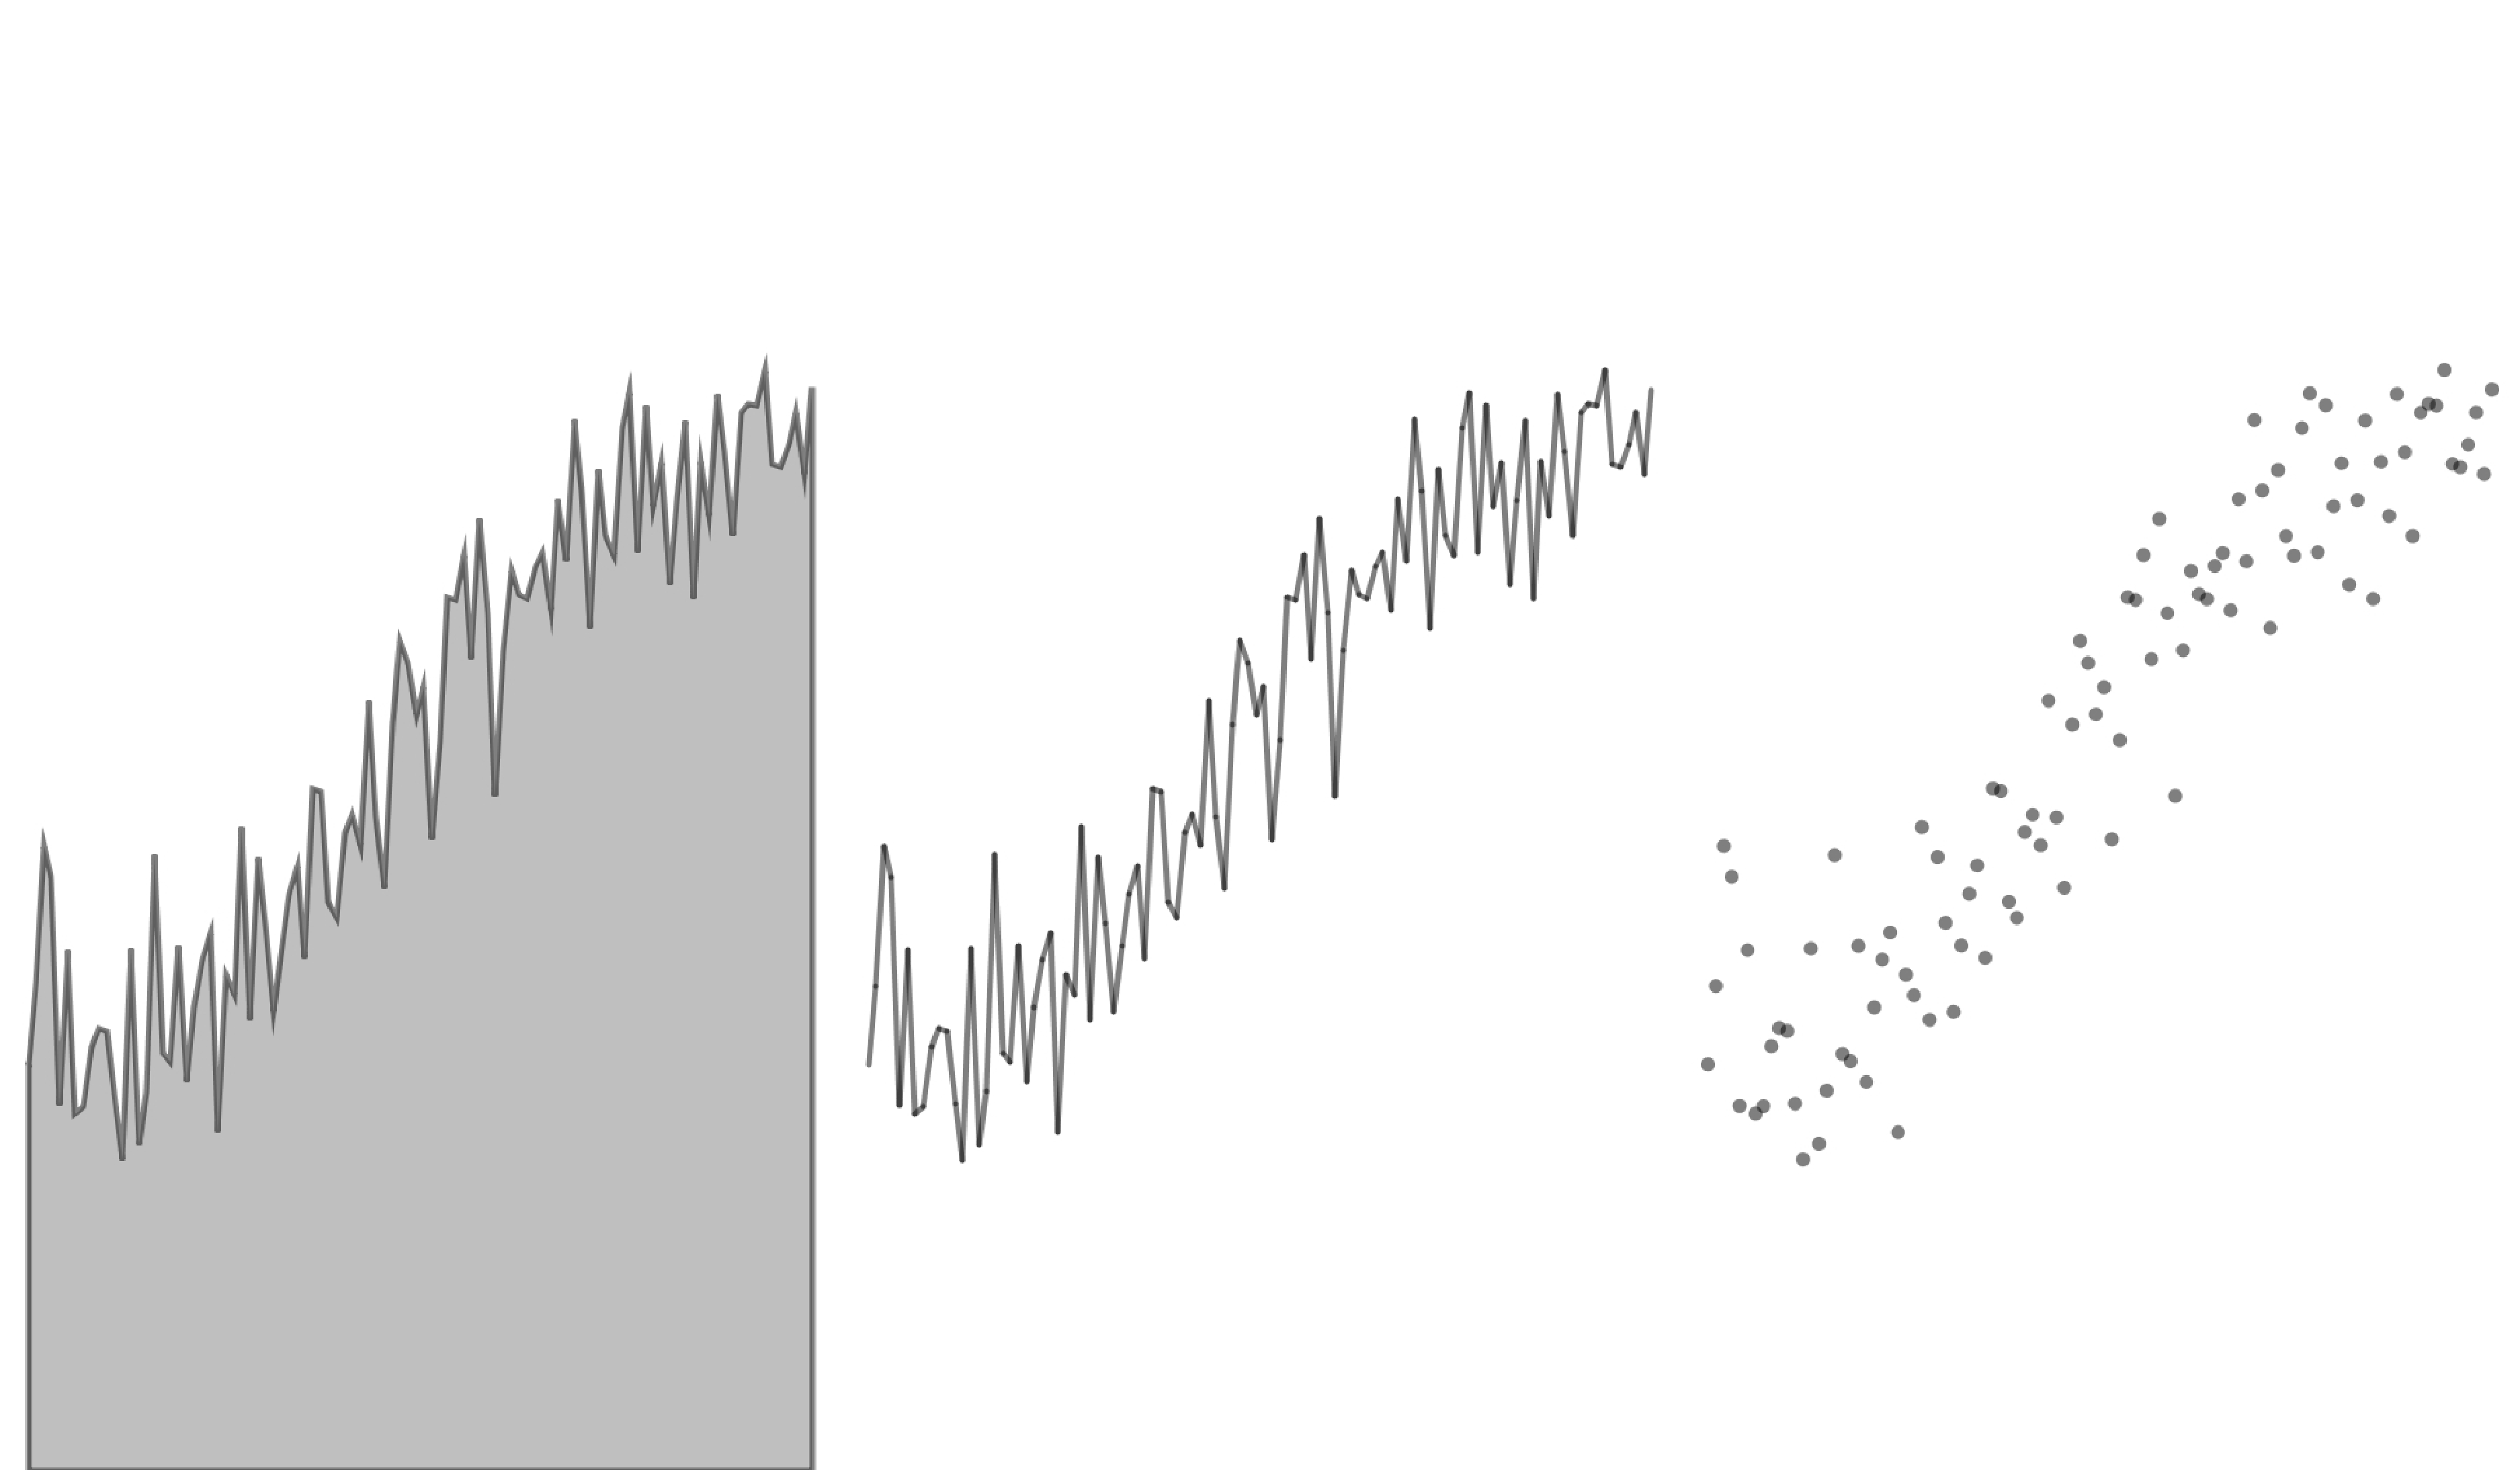
\includegraphics[width=.95\columnwidth]{figures/types}
		\caption{The three types of bivariate visualizations explored in this work: area charts, line charts, and scatterplots. The density of points made bar charts and area charts extremely visually similar, and so they were excluded from our experiments. Likewise, the error in estimating trends from heatmaps\protect\cite{fuchs2013evaluation} made them unsuitable for the experimental task.}
		\label{fig:types}
	\end{figure}
}

\newcommand{\expTwoTypesFig}{
	\begin{figure}
		\centering
		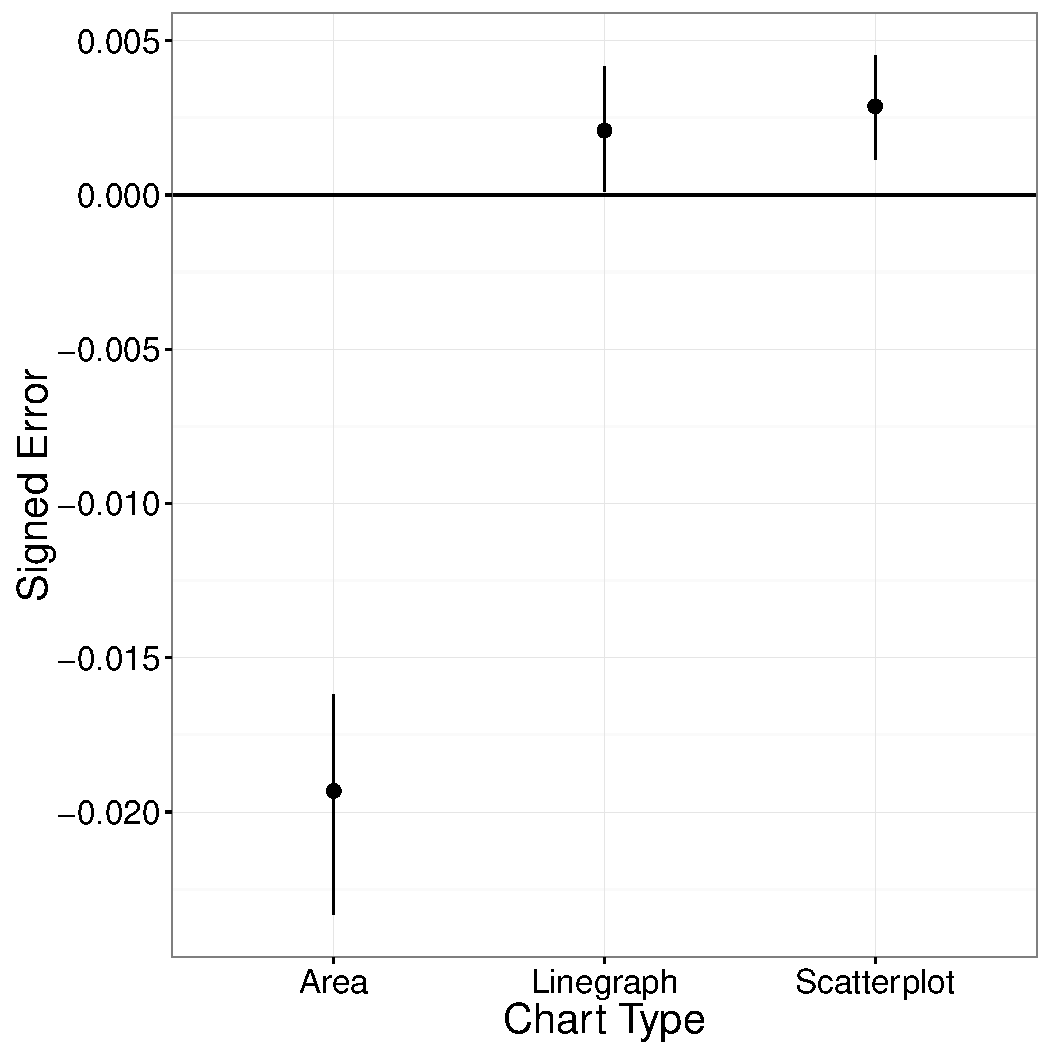
\includegraphics[width=.85\columnwidth]{figures/exp2types}
		\caption{From experiment 2, the effect of chart type on signed error. See Fig. \protect\ref{fig:sigmas} for example stimuli at each factor level. Area charts are visually asymmetric, with the area below the line filled in with a color. This visual asymmetry results in a form of within-the-bar bias\protect\cite{newman2012bar}, where values in the filled region are perceived as likelier than values outside of it. This bias manifests as a consistent underestimation in the intercept of trend lines. Other chart types we examined do not have this bias. Confidence intervals represent bootstrapped 95\% c.i.s of interquartile mean. }
		\label{fig:exp2types}
	\end{figure}
}
